\chapter{Setting Up}

In this chapter we describe the environment we use to do our test, the tool

\section{Python environment}
The language used to interface with quantum computer is usually python, in this section we create a virtual environment in python in order to communicate with the IBM quantum Computer and the D-Wave quantum computer.

For our test we manage pyton environments with \mintinline{sh}|conda|, let's start creating the virtual env named \mintinline{sh}|quantum| and activate it with:
\begin{minted}{sh}
conda create --name quantum python=3.12 pip
conda activate quantum
\end{minted}
For our test and to follow the various example presented both by IBM and D-Wave is also useful to been able of running a Jupyter notebook. We can install Jupyter with:
\begin{minted}{sh}
pip install jupyter
\end{minted}

\section{IBM Qiskit}
To program an architecture gate based and to access IBM quantum computer we use the \emph{Qiskit} software stack. The name Qiskit is a general term referring to a collection of software for executing programs on quantum computers.
\begin{figure}[h]
	\centering
	\includegraphics[width=.95\linewidth]{overview-image}
	\label{fig:qiskit_overview}
	\caption{Qiskit software stack}
\end{figure}

The core components are \emph{Qiskit SDK} and \emph{Qiskit Runtime}, the first one is completely open source and allows the developer to define his circuit; the second one is a cloud-based service for executing quantum computations on IBM quantum computer.

\subsection{Hello World}
Following the IBM documentation\footnote{https://quantum.cloud.ibm.com/docs/en/guides/install-qiskit} we can install the SDK and the Runtime with:
\begin{minted}{sh}
pip install qiskit matplotlib qiskit[visualization]
pip install qiskit-ibm-runtime
pip install qiskit-aer
\end{minted}

Line $3$ install Aer, that is a high performance simulator for quantum circuits written in Qiskit. Aer includes realistic noise models, and we will use later to test our circuit.

Sometimes the Qiskit stack suffer from incompatibility between the various software that compose the environment. At the moment of writing the latest package seem to work without any problem. For our test we will use \mintinline{py}|qiskit: 2.2.3|, \mintinline{py}|qiskit-ibm-runtime: 0.43.1| and \mintinline{py}|qiskit-aer: 0.17.2|.

If the setup had success we are now able to run a small test to build a Bell state (two entangled qubits). The following code assemble the gates, show the final circuit and use a sampler to simulate on the CPU the result of $1024$ runs of the program.

\begin{listing}[H]
	\begin{minted}{py}
from qiskit import QuantumCircuit
from qiskit.primitives import StatevectorSampler

qc = QuantumCircuit(2)
qc.h(0)
qc.cx(0, 1)
qc.measure_all()

sampler = StatevectorSampler()
result = sampler.run([qc], shots=1024).result()
print(result[0].data.meas.get_counts())
qc.draw("mpl")
	\end{minted}
	\label{lst:hello_qiskit}
	\caption{hello qiskit}
\end{listing}

\subsection{Transpilation}
Each Quantum Processing Unit (QPU) has a specific topology, we need to rewrite our quantum circuit in order to match the topology of the selected device on witch we want to run our program. This phase of rewriting, followed by an optimization, is called transpilation. 

Considering, for now, a fake hardware (so we don't need an API key) we can transpile the quantum circuit \mintinline{py}|qc|, from the code above, to match the topology of a precise QPU:
\begin{listing}[H]
	\begin{minted}{py}
from qiskit_ibm_runtime.fake_provider import FakeWashingtonV2
from qiskit.transpiler import generate_preset_pass_manager

backend = FakeWashingtonV2()
pass_manager = generate_preset_pass_manager(backend=backend)

transpiled = pass_manager.run(qc)
transpiled.draw("mpl")
	\end{minted}
	\label{lst:transpilation}
	\caption{Transpilation}
\end{listing}
The following picture show (\ref{fig:qc_orig}) the quantum circuit that build a Bell state, and (\ref{fig:qc_trans}) the transpiled version where the Hadamard gate is replaced to match the actual topology of the QPU.
\begin{figure}[h]
	\centering
	\subfloat[Original circuit]
	{\label{fig:qc_orig}
		\includegraphics[height=2.8cm]{bell_1}} \quad
	\subfloat[Transpiled circuit]
	{\label{fig:qc_trans}%
		\includegraphics[height=2.8cm]{bell_2}} \\
	\label{fig:qc_transpilation}
	\caption{Transpilation example}
\end{figure}


\subsection{Execution}
To test our transpiled circuit we use Aer that allow us to simulate also the noise of a real quantum hardware. We can execute our program with:
\begin{listing}[H]
	\begin{minted}{py}
from qiskit_aer.primitives import SamplerV2

sampler = SamplerV2.from_backend(backend)
job = sampler.run([transpiled], shots=1024)
result = job.result()
print(f"counts for Bell circuit : {result[0].data.meas.get_counts()}")
	\end{minted}
	\label{lst:execution}
	\caption{Simulated execution}
\end{listing}

If we look at the results of the execution we could observe that some answers present non entangled qbit, this is caused by the (simulated) noise of the quantum device. A typical output of the execution could be:
\begin{minted}{text}
> counts for Bell circuit : {'00': 504, '11': 503, '01': 10, '10': 7}
\end{minted}
Where state \mintinline{text}|01| and \mintinline{text}|10| should not be present in an ideal execution with no errors.

\subsection{A complete example on real hardware}

\section{D-Wave Ocean}
To define an optimization problem that can be resolved on a D-Wave quantum computer we use the Ocean software stack. Ocean, also, allow us  to interact with D-Wave hardware, submit a problem and to simulate the execution on a classical CPU.
\begin{figure}[h]
	\centering
	\includegraphics[width=.95\linewidth]{ocean_stack}
	\label{fig:ocean_overview}
	\caption{Ocean software stack}
\end{figure}

All tools that implement the steps needed to solve your problem on a CPU, a D-Wave quantum computer, or a quantum-classical hybrid solver can be installed with:
\begin{minted}{sh}
pip install dwave-ocean-sdk
\end{minted}

After the installation running the command \mintinline{sh}|dwave setup| will start an interactive prompt that guide us through a full setup. During the setup is also possible adding a API token or connecting to the D-Wave account to import directly a key to use the quantum hardware.
\subsection{Hello World}
To present simple optimization program we consider the minimum vertex cover (MVC) problem. Given a graph $G = (V, E)$ the problem asks to find a subset $V'\subseteq V$ that for each edge $\set{u,v} \in E$ at least one of $v$ or $u$ belongs to $V'$ and the number of nodes in $V'$ ($|V'|$) is the lowest possible.

The reduction from MVC to Ising formulation is well known, the cost function, that we want to minimize, could be expressed by:
\[
cost = \sum_{i = 1}^{|V|}v_i + 2 \cdot \sum_{\set{i,j} \in E}\left(1-v_i-v_j+v_iv_j\right)
\]
Where $v_i \in \set{-1, 1}$ and if $v_i = 1$ means that $v_i \in V'$, otherwise  $v_i = -1$. 

Like all problem in Ising form we can express the cost as a symmetrical matrix, so our function become 
\[
cost = v^T\times \mathbf{M}\times v
\]
Were $v$ is the vector containing the binary variables $v_i$.

The figure shows an example graph (\ref{fig:ising_ex_gr}) and the corresponding matrix (\ref{fig:ising_ex_mx}) expressing the cost function.

\begin{figure}[h]
	\centering
	\subfloat[Original graph]
		{\label{fig:ising_ex_gr}
			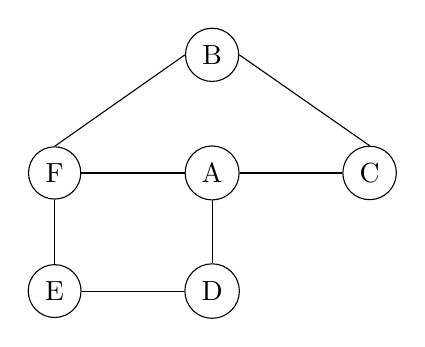
\begin{tikzpicture}
				\node (a) at (0,0)        [draw, circle] {A};
				\node (b) at (0,1.5)      [draw, circle] {B};
				\node (c) at (2,0)         [draw, circle] {C};
				\node (d) at (0,-1.5)     [draw, circle] {D};
				\node (e) at (-2,-1.5)    [draw, circle] {E};
				\node (f) at (-2,0)			[draw, circle] {F};
				\draw[-] (a.east)  -- (c.west);
				\draw[-] (a.south) -- (d.north);
				\draw[-] (a.west) -- (f.east);
				\draw[-] (b.east) -- (c.north);
				\draw[-] (b.west) -- (f.north);
				\draw[-] (d.west) -- (e.east);
				\draw[-] (e.north) -- (f.south);
			\end{tikzpicture}
		} \qquad
	\subfloat[Corresponding matrix]
		{
			\label{fig:ising_ex_mx}%
			\begin{tikzpicture}
				\node (a) at (0,0) {
					$
					\mathbf{M} = 
					\begin{pmatrix}
						1&0&2&2&0&2\\
						0&1&2&0&0&2\\
						0&0&1&0&0&0\\
						0&0&0&1&2&0\\
						0&0&0&0&1&0\\
						0&0&0&0&0&1\\
					\end{pmatrix}
					$
				};
			\end{tikzpicture}
		}
	\label{fig:ising_ex}
	\caption{Ising formulation}
\end{figure}

The following code present a possible implementation of the Ising model described above. We have defined two dictionary to memorize the matrix coefficient. The last line of code founds ten possible answers to the problem using the simulated annealing function implemented by D-Wave.
\begin{listing}[H]
	\begin{minted}{py}
from dwave.samplers import SimulatedAnnealingSampler
linear = {'A': 1, 'B': 1, 'C': 1, 'D': 1, 'E': 1, 'F': 1}
quadratic = {('B', 'C'): 2, ('B', 'F'): 2, ('C', 'A'): 2, ('D', 'A'): 2, ('E', 'D'): 2, ('E', 'F'): 2, ('F', 'A'): 2}
sampler = SimulatedAnnealingSampler()
result = sampler.sample_ising(linear, quadratic, num_reads=10)
	\end{minted}
	\label{lst:ising_ex}
	\caption{Ising example}
\end{listing}
If we print the results with: \mintinline{py}|print(result.aggregate())| we could observe something similar to this:
\begin{minted}{text}
	A  B  C  D  E  F energy num_oc.
0 -1 -1 +1 +1 -1 +1  -14.0       6
1 +1 +1 -1 -1 +1 -1  -14.0       4
['SPIN', 2 rows, 10 samples, 6 variables]
\end{minted}
The two different results represent the two correct answer to our particular instance of the MVC problem.

\subsection{Example on real hardware}

\subsection{Minor embedding}

\section{PyQubo and QuboVert}
In listing \ref{lst:ising_ex} we have manually built the matrix representing the function that we want to minimize. It can be useful to have some tools that allow us working at higher level defining the function like:
\[
	cost = objective + \lambda \cdot penalty
\]


